% \frame{\frametitle{The DRDoS attack}
% \begin{columns}
%   \begin{column}{0.6\textwidth}
%     \includegraphics[width=1\linewidth]{../image/drdos_1.pdf}
%   \end{column}
%   \begin{column}{0.4\textwidth}
%     \begin{itemize}
%     \item Attacker identifies a vulnerable service
%     \item Attacker sends requests to the service spoofing the IP to appear to be the victim
%     \end{itemize}
%   \end{column}
% \end{columns}
% }




\begin{frame}
	\frametitle{ Table of Contents}
	\begin{itemize}
		\item Introduction
		\item Automation and Labor
		\begin{itemize}
			\item Net Impact on Job Market
			\item Solutions to Impeding Problems
		\end{itemize}
		\item Ethical Questions in Automation
		\begin{itemize}
			\item Responsibility in Automated Systems
			\item Trust in Automated Systems
		\end{itemize}
		\item Questions
	\end{itemize}
\end{frame}


\begin{frame}
	\frametitle{ Ethical Automation: Introduction}
	\begin{itemize}
		\item A note on Labor
		\item A brief review of the industrial revolution(s)
		\item The Big Questions:
		\begin{itemize}
			\item We know automation destroys jobs.  How many does it make?
			\item What do we do when people lose their jobs?
		\end{itemize}
	\end{itemize}
\end{frame}


\begin{frame}
  \frametitle{ Ethical Automation: will automation create net job loss?}
  {\Large History tells us otherwise}
\end{frame}

\begin{frame}
	\frametitle{Ethical Automation: will automation create net job loss?}
	
	\begin{figure}[bht]
	\centering
	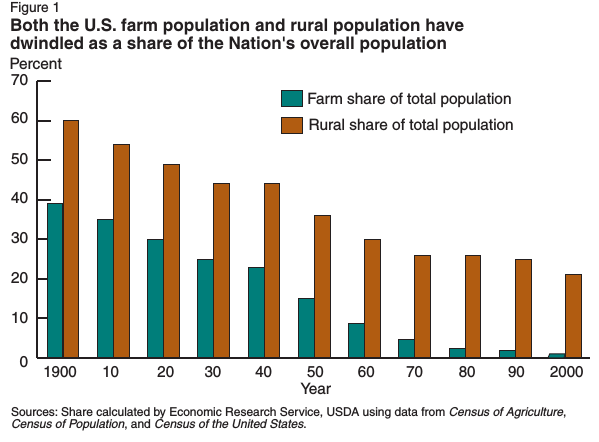
\includegraphics[scale=0.5]{diagrams/agriculture-data}
	\end{figure}
	\textit{Source:Dimitri,Effland, and Conklin. The 20th century transformation of US agriculture and farm policy.}
	
\end{frame}

\begin{frame}
	\frametitle{Ethical Automation: will automation create net job loss? }
	{\Large But surprisingly..}
	\begin{figure}[bht]
	\centering
	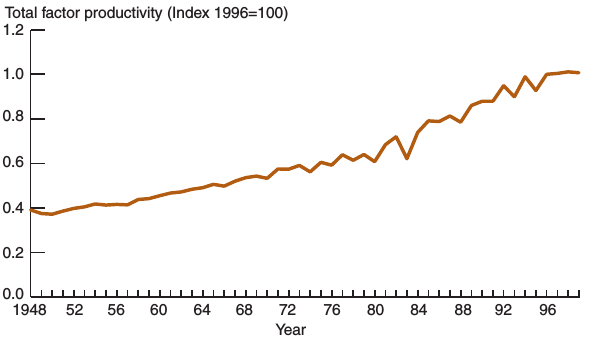
\includegraphics[scale= 0.4]{diagrams/agriculture-production}
	\end{figure}
	\textit{Source:Dimitri,Effland, and Conklin. The 20th century transformation of US agriculture and farm policy.}
\end{frame}

\begin{frame}
	\frametitle{Ethical Automation: will automation create net job loss? }
	{\Large And even more astonishingly exports went up!}
	\begin{figure}[bht]
	\centering
	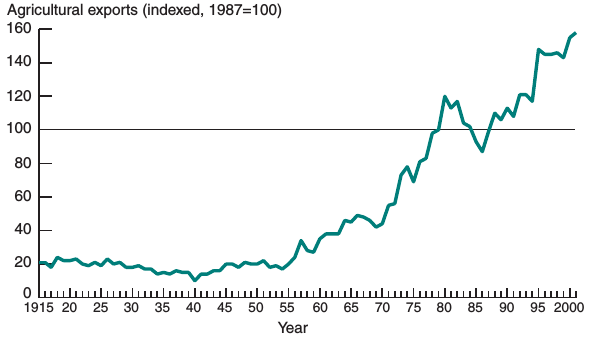
\includegraphics[scale= 0.4]{diagrams/agriculture-exports}
	\end{figure}
	\textit{Source:Dimitri,Effland, and Conklin. The 20th century transformation of US agriculture and farm policy.}
\end{frame}

\begin{frame}
	\frametitle{Ethical Automation: will automation create net job loss? }
	{\Large What type of jobs are automated?}
	\begin{itemize}
	\item Human work that is very labor intensive
	\item repetitive in nature
	\item Largely, not a creative process. 
	\end{itemize}
\end{frame}

\begin{frame}
	\frametitle{Ethical Automation: will automation create net job loss? }
	{\Large Automation reduces cost.}
	\begin{itemize}
	\item Normally calculated using a Cost- Based Analysis
	\item Improves efficiency
	\item ..in turn improving production
	\item but wait there's more...!
	\end{itemize}
\end{frame}

\begin{frame}
	\frametitle{Ethical Automation: will automation create net job loss? }
	{\Large Improves quality of life}
	\begin{itemize}
	\item One of the primary pros of automation is the freeing up of time for leisure.
	\item  We have seen a 20 \% reduction in work hours from the start of the 20th century to it's end.
	\item This has left people to pursue more interesting job prospects.
	\end{itemize}
\end{frame}
\begin{frame}
\frametitle{Ethical Automation: proposed solutions to job loss}
{\Large Is there a need for a solution?}
\end{frame}

\begin{frame}
\frametitle{Ethical Automation: proposed solutions to job loss}
{\Large Tl;DR. No.}
\end{frame}
\begin{frame}
	\frametitle{Ethical Automation: will automation create net job loss? }
	{\Large Long Answer.}
	\begin{itemize}
	\item According to a study carried out by economists at Deloitte UK LLP, using close to 140 years of census data from Wales and Britain.
	\item Here are some of the results of the study
	\end{itemize}
\end{frame}
\begin{frame}
	\frametitle{Ethical Automation: will automation create net job loss? }
	\begin{figure}[th]
	\centering
	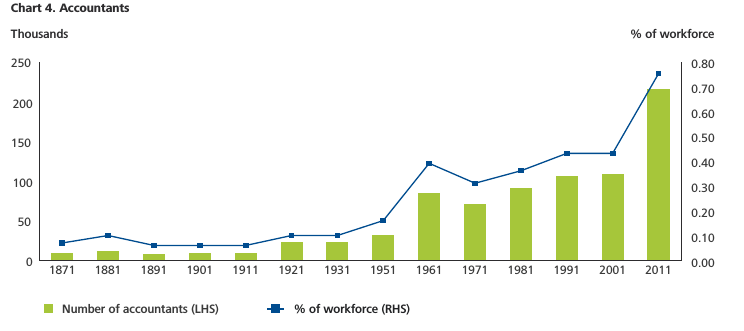
\includegraphics[scale=0.3]{diagrams/accountants-growth}
	\end{figure}
	\begin{figure}[h]
		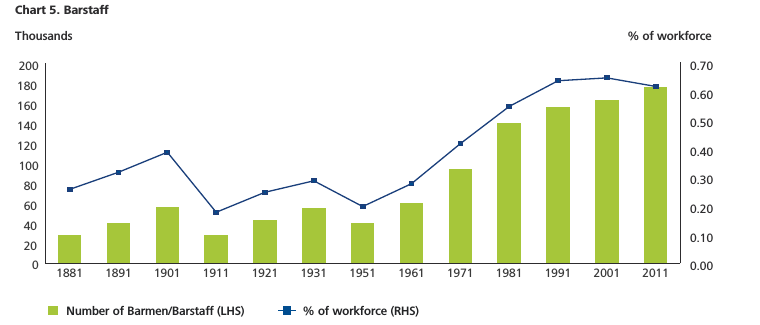
\includegraphics[scale=0.3]{diagrams/barstaff-growth}
		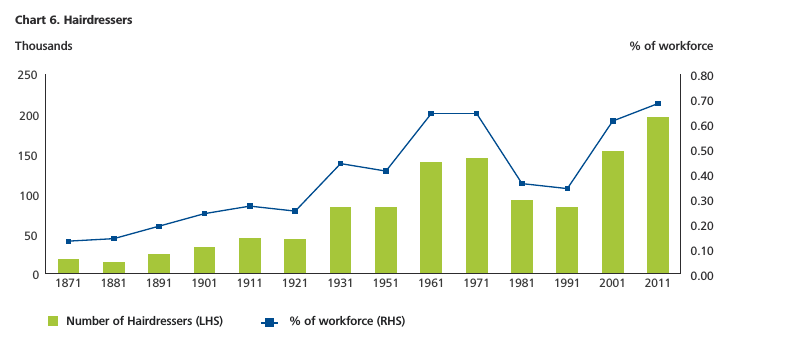
\includegraphics[scale=0.3]{diagrams/hairdressers-growth}
	\end{figure}
\end{frame}

\begin{frame}
	\frametitle{Ethical Automation: will automation create net job loss? }
	{\Large The situation as it stands now}
	\begin{itemize}
	\item We stand at a unique position now, where we are seeing computational power growing rapidly
	\item We are seeing accessibility to services improving.
	\item Manage appointments, remember birthdays, suggest restaurants, suggest best possible routes, plan a vacation
	\item All of the above would require a whole lot of human effort and time to do, today we have apps that do this for us. 
	\item We are slowly seeing a shift from simply menial manual work, but mental work. Some would argue this is a significant paradigm shift.
	
	\end{itemize}
\end{frame}
\begin{frame}
	\frametitle{Ethical Automation: will automation create net job loss? }
	{\Large Amazon's Robot Army and the Human- Machine Symbiosis}
	\begin{itemize}
	\item In 2012, Amazon acquired Kiva Systems, that produces the robots that now operate most of amazon's warehouses in the United States
	\item .."Coincidentally or not, Amazon bought Kiva soon after a press report revealed that workers at one of the retailer’s giant warehouses often walked more than 10 miles a day."
	\item Although, this might have led to some jobs being lost. There is still a requirement for human intervention
	\item Packaging, selecting and various other tasks still require a human to do.
	\item And the robot is merely a tool.
	\item ..this is not very different from what happened during the first machine age
	\end{itemize}
\end{frame}

\begin{frame}
	\frametitle{Ethical Automation: will automation create net job loss? }
	{\Large In conclusion..}
	\begin{itemize}
	\item There is still division amongst economists about whether this is similar to the previous industrial age
	\item some believe that with more automation of mental activities, we are going to see a sharp decline in 'good-middle class' jobs
	\item Agreement across the board, that apps taking away knowledge jobs, but it is too early to predict what will happen with certainty.
	\item One thing is for sure, we are definitely in unchartered territory, the only question is whether it will follow trends we have seen earlier or will it set new trends is yet to be seen.
	\end{itemize}
\end{frame}


\begin{frame}
	\frametitle{ Ethical Automation: proposed solutions to job loss}
	\begin{itemize}
		\item
	\end{itemize}
\end{frame}

\begin{frame}
	\frametitle{ Ethical Automation: A brief aside}
	\begin{itemize}
		\item From Worker to Product
		\begin{itemize}
			\item We've talked about a worker being replaced by a machine
			\item How do we talk about those machines?
		\end{itemize}
		\item What is Responsibility?
		\item The Big Questions:
		\begin{itemize}
			\item When an automated machine fails, who is responsible?
			\item What kind of failure is acceptable?
		\end{itemize}
	\end{itemize}
\end{frame}


\begin{frame}
	\frametitle{ Ethical Automation: Responsibility in Automation}
	\Large{Responsiblity}
\end{frame}


\begin{frame}
	\frametitle{ Ethical Automation: Responsibility in Automation}
	{\Large Self-Driving Cars}
	\begin{itemize}
		\item The manufacturer is liable for failure, not the user
	\end{itemize}
\end{frame}


\begin{frame}
	\frametitle{ Ethical Automation: Responsibility in Automation}
	{\Large How Safe is Safe Enough?}\\
	424,331 autonomous miles. . . with a catch
	\begin{itemize}
		\item ``Safety Driver''
		\item Relinquished Control
		\item Emergency Intervention
	\end{itemize}
\end{frame}


\begin{frame}
	\frametitle{ Ethical Automation: Trust in Automation}
	\Large{Is it Moral to Trust the Morality of a Machine?}
\end{frame}


\begin{frame}
	\frametitle{ Ethical Automation: Trust in Automation}
	\begin{figure}[bht]
		\centering
		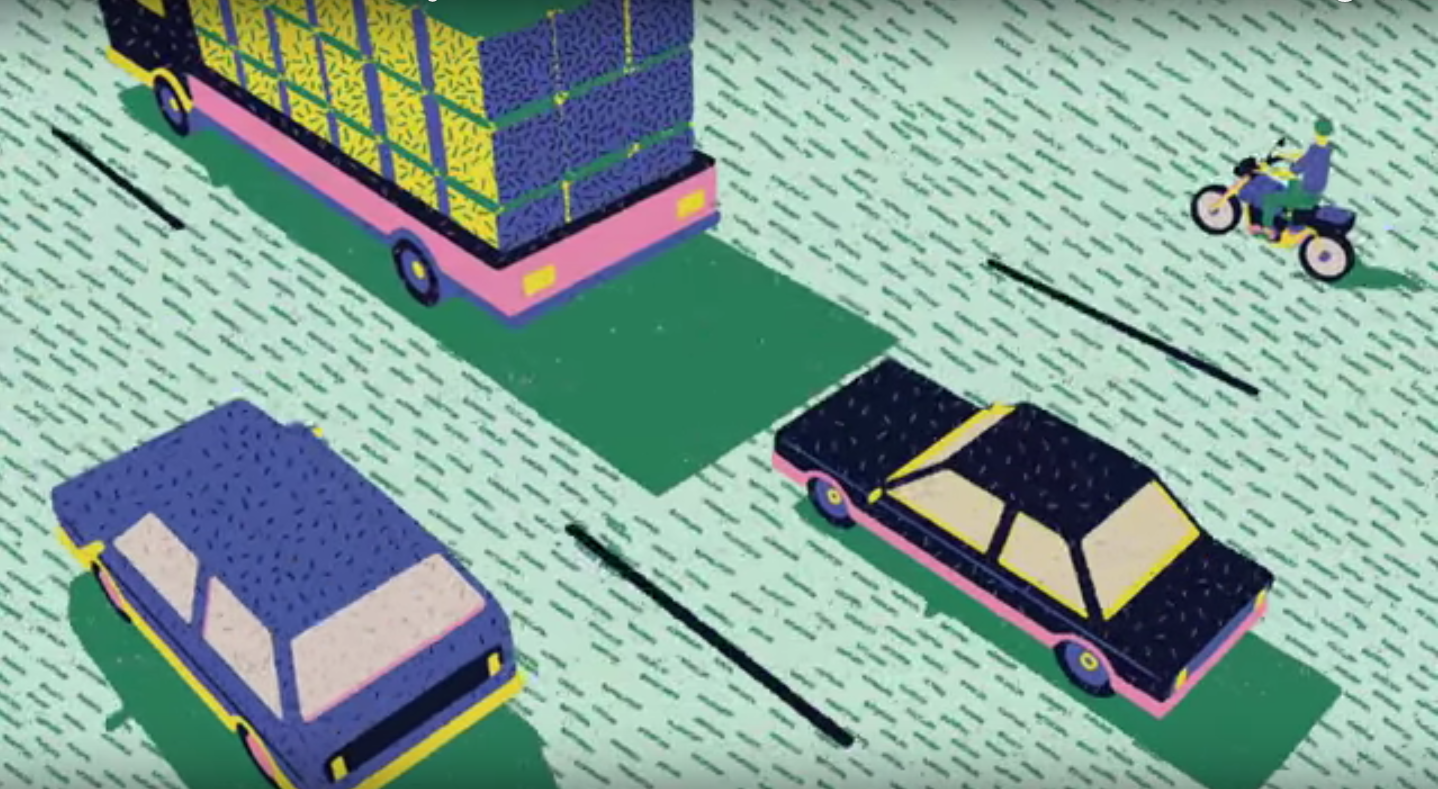
\includegraphics[width=4.1in]{diagrams/image00}
		\caption{An Ethical Scenario.}
		\label{fig:-deg}
	\end{figure}
\end{frame}


\begin{frame}
	\frametitle{ Ethical Automation: Trust in Automation}
	{\Large Reaction vs Decision}
	\begin{itemize}
		\item Humans react while machines decide
	\end{itemize}
\end{frame}


\begin{frame}
	\frametitle{ Ethical Automation: Trust in Automation}
	\begin{figure}[bht]
		\centering
		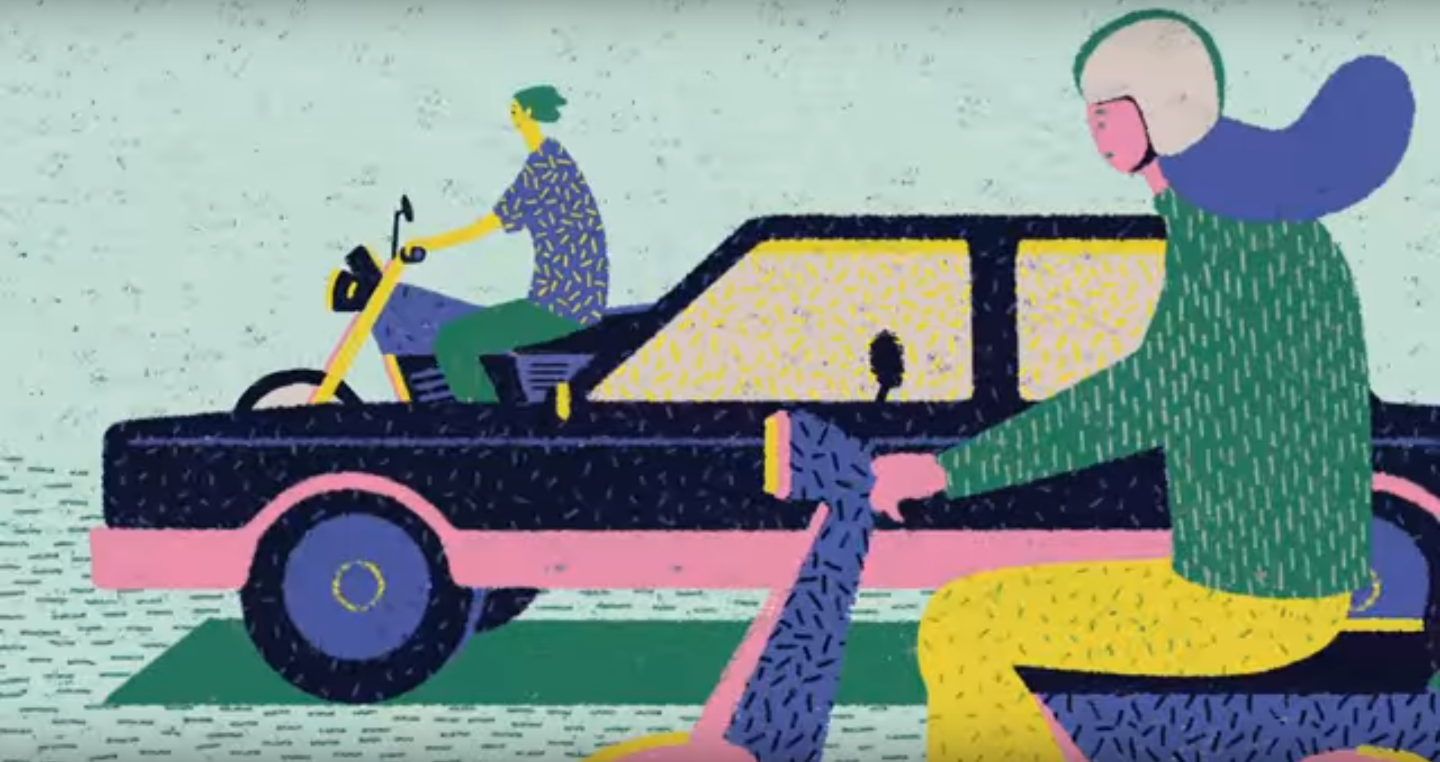
\includegraphics[width=4.1in]{diagrams/image01}
		\caption{}
		\label{fig:-deg}
	\end{figure}
\end{frame}


\begin{frame}
	\frametitle{ Ethical Automation: Trust in Automation}
	{\Large Conclusion}
	\begin{itemize}
		\item These moral dilemmas are too complicated and too controversial to decide
	\end{itemize}
\end{frame}


\begin{frame}
	\frametitle{ Ethical Automation: Trust in Automation}
	\begin{itemize}
		\item
	\end{itemize}
\end{frame}


\begin{frame}
	\frametitle{ Ethical Automation: Responsibility in Automation}
	{\Large Self-Driving Cars}
	\begin{itemize}
		\item Do you watch cop shows, crime drama and action flicks?
	\end{itemize}
\end{frame}

\begin{frame}
	\frametitle{ Ethical Automation: Responsibility in Automation}
	{\Large Reaction time!}
	\begin{itemize}
		\item Human reaction time is 2.3 seconds
		\item Airplane 45 seconds
		\item Car 2.3 seconds
	\end{itemize}
\end{frame}

\begin{frame}
	\frametitle{ Ethical Automation: Responsibility in Automation}
	{\Large This is not enough time for;}
	\begin{itemize}
		\item A human to realize something is wrong.
		\item Decide what to do
		\item Take over control
		\item Take action
	\end{itemize}
\end{frame}

\begin{frame}
	\frametitle{ Ethical Automation: Trust in Automation}
	{\Large Driver or AI?}
	\begin{figure}[bht]
		\centering
		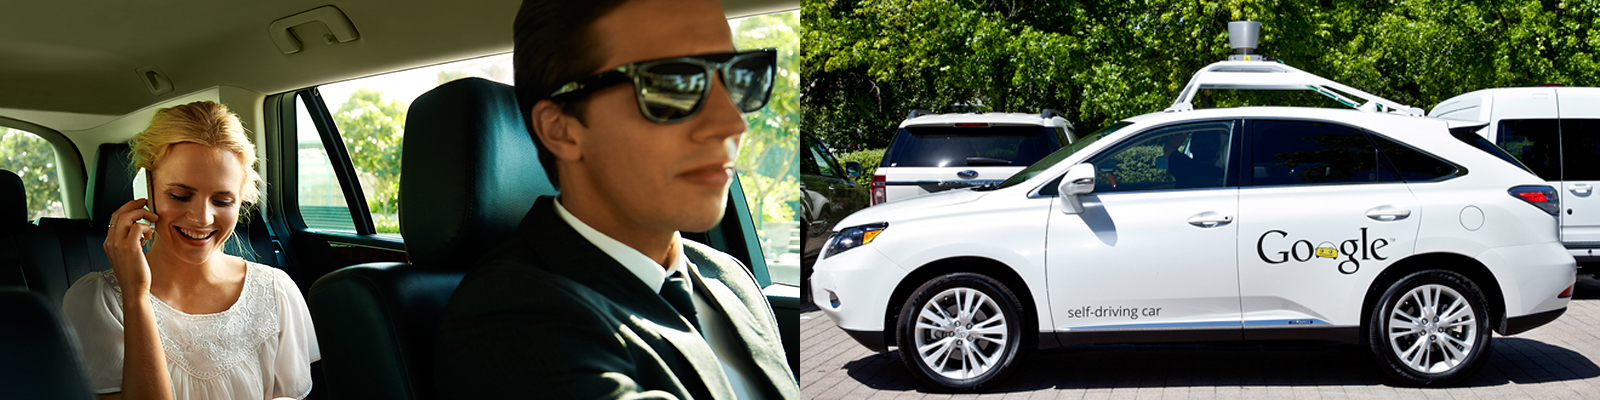
\includegraphics[width=4.1in]{diagrams/car}
		\caption{}
		\label{fig:-deg}
	\end{figure}
\end{frame}

\begin{frame}
	\frametitle{ Ethical Automation: Trust in Automation}
	{\Large Mass paranoia?}
	\begin{figure}[bht]
		\centering
		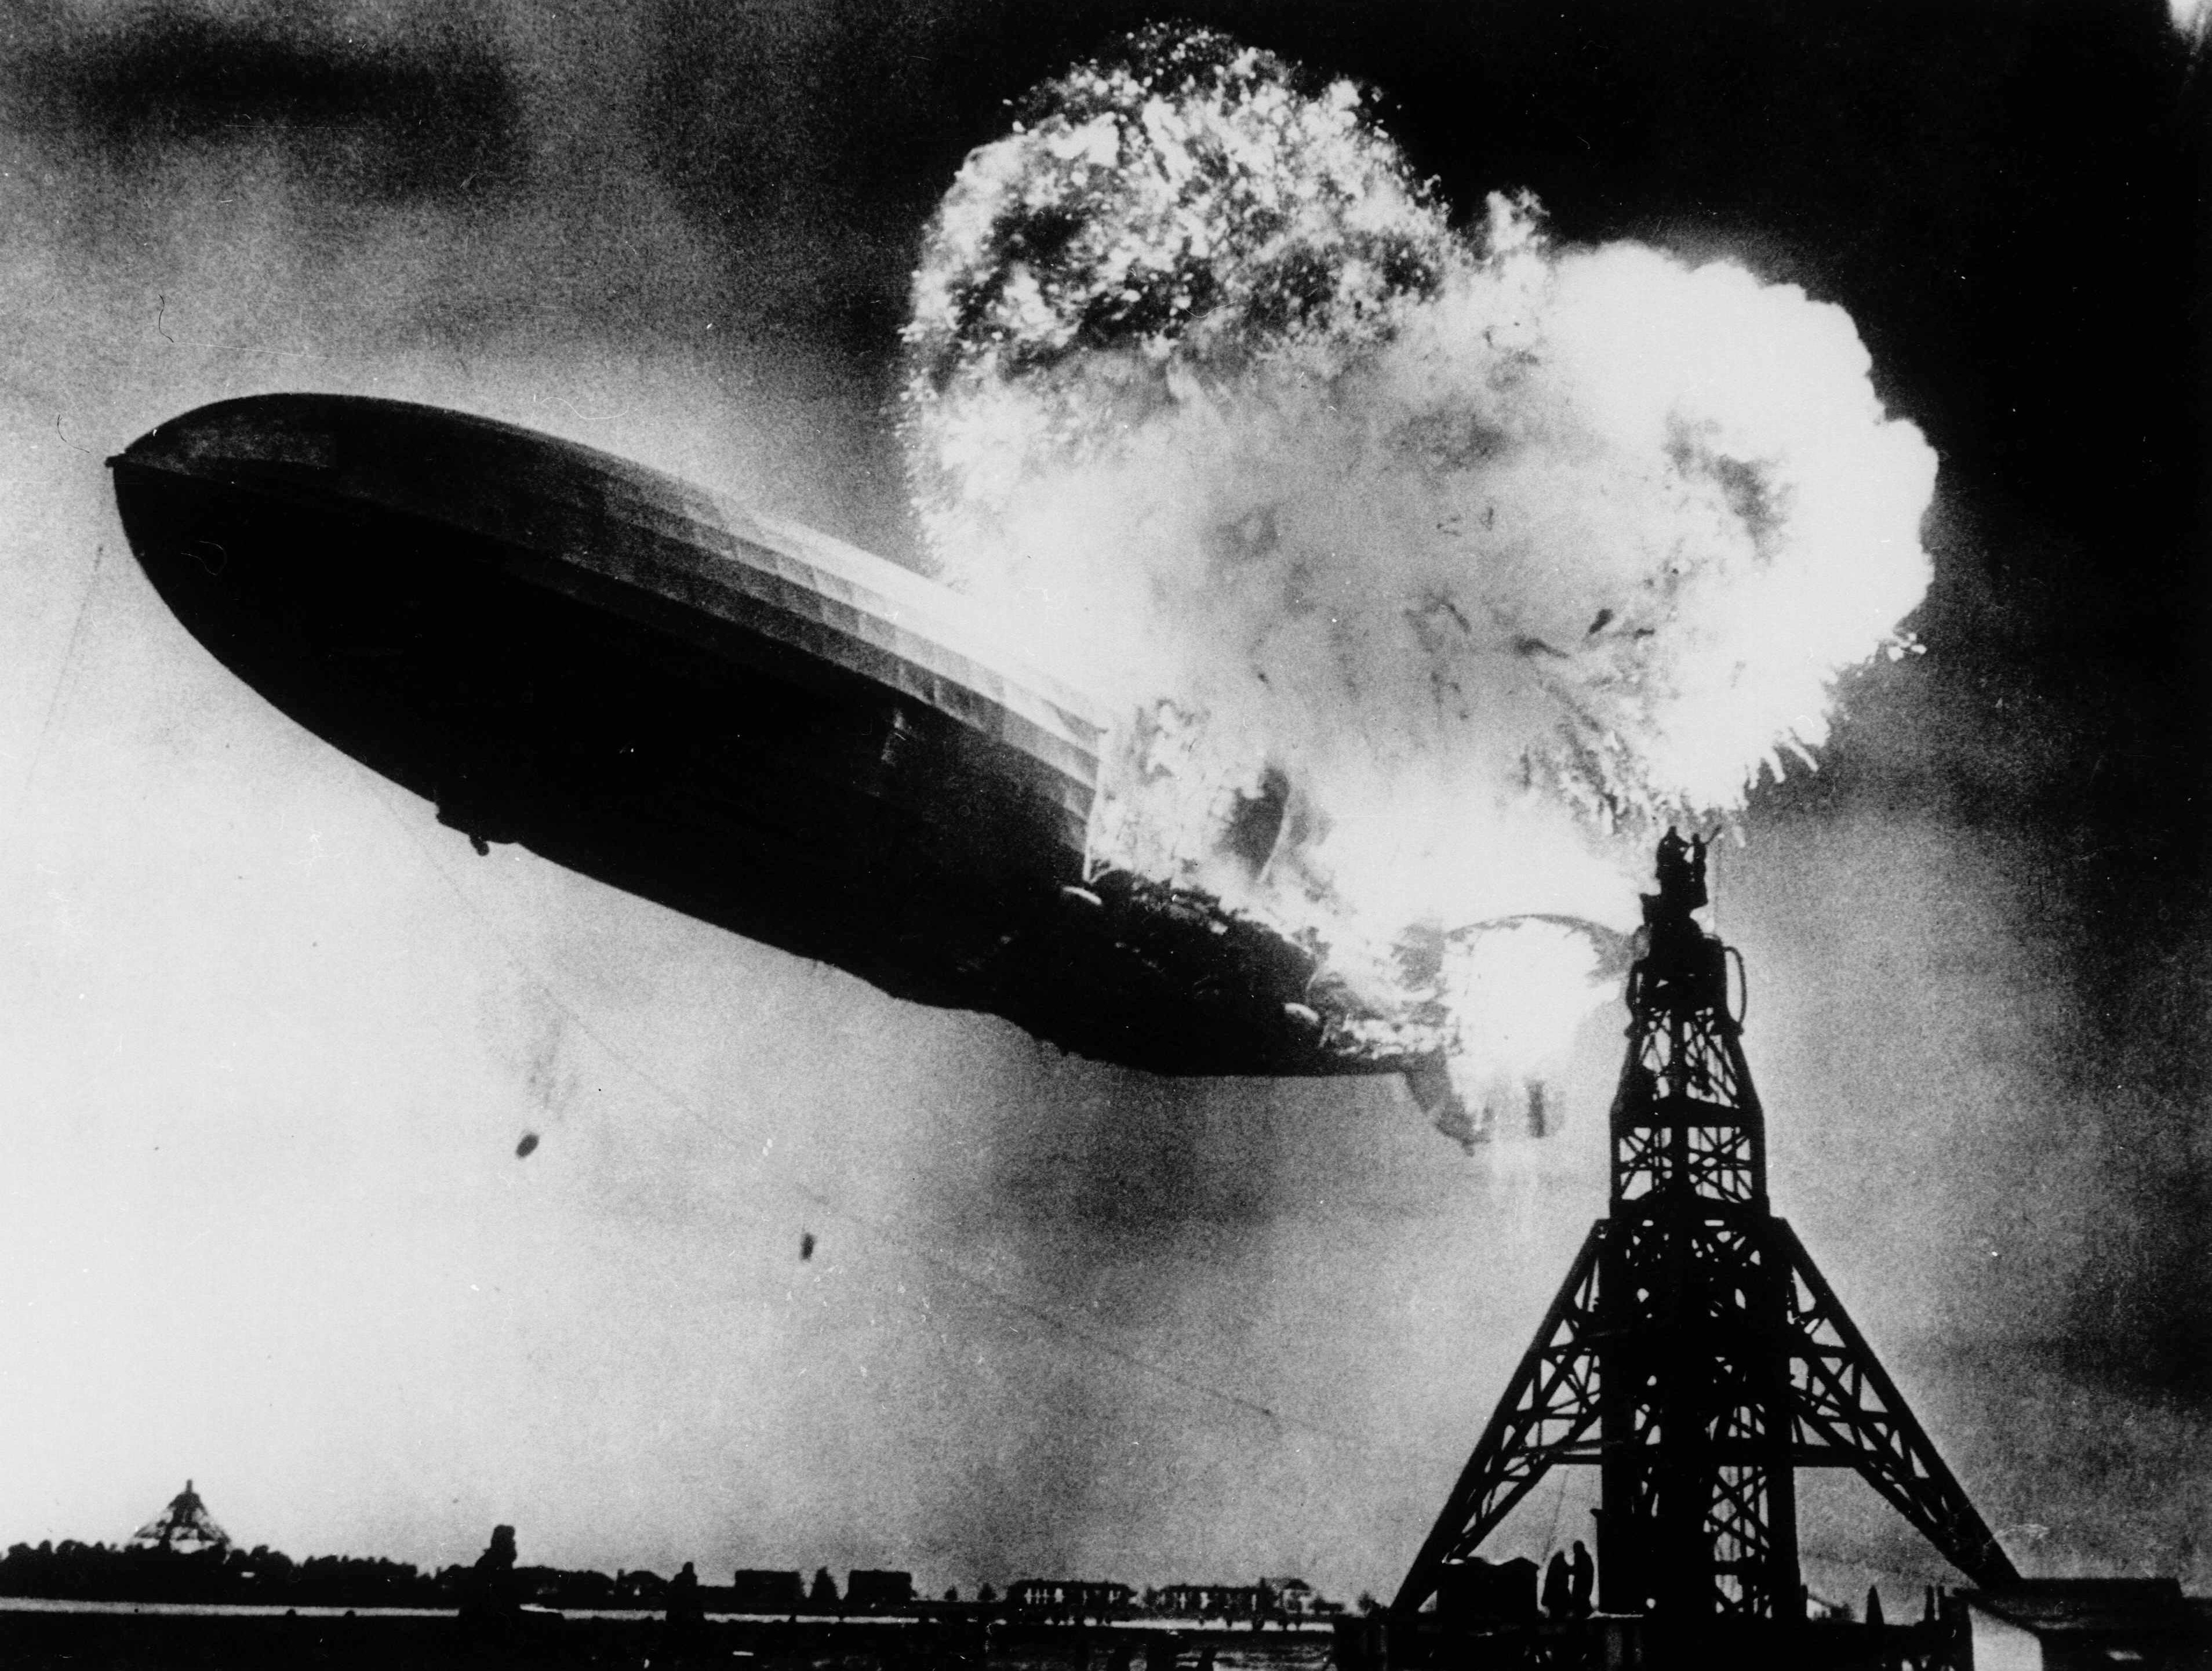
\includegraphics[width=4.1in]{diagrams/Hindenburg}
		\caption{}
		\label{fig:-deg}
	\end{figure}
\end{frame}

\begin{frame}
	\frametitle{ Ethical Automation: Trust in Automation}
	{\Large Are we asking the right questions?}
	\begin{figure}[bht]
		\centering
		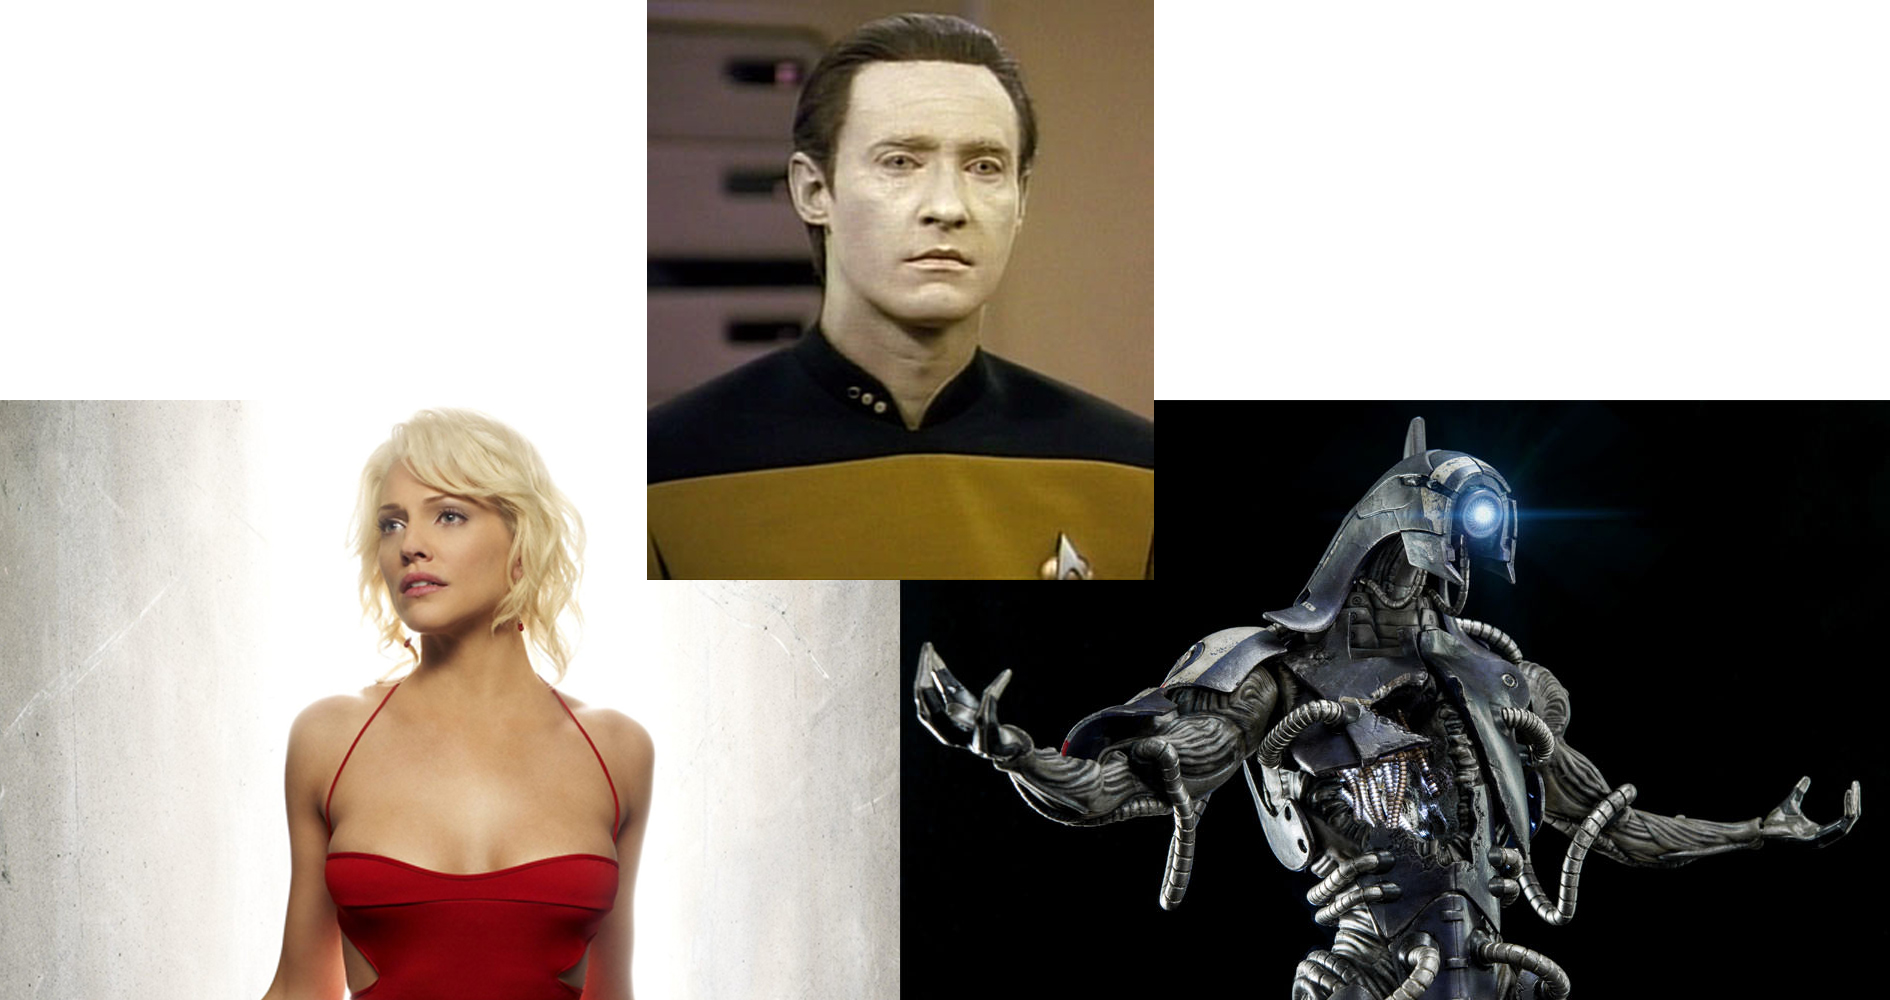
\includegraphics[width=4.1in]{diagrams/AIs}
		\caption{}
		\label{fig:-deg}
	\end{figure}
\end{frame}

\begin{frame}
	\frametitle{ Ethical Automation: Conclusion}
	\begin{itemize}
		\item Consequences of automation
		\item Big changes are coming
		\begin{itemize}
			\item We've got to talk about it now,
			\item We've got to to talk about it a lot.
		\end{itemize}
	\end{itemize}
\end{frame}


\begin{frame}
	\frametitle{ Ethical Automation: Conclusion}
	\Large Questions?
\end{frame}
